\section{Montel's Theorem}\label{appendixmontel}

In Section \ref{complexdynamics} we discussed the equivalence between equicontinuity and normality in $\C$. Here we explore another useful condition which implies normality in open subsets of $\mathbb{C}$.


\begin{mydef}{}{}
A family of analytic functions $\{f_i\}_{i\in I}$ defined in a domain $\Omega \subset \mathbb{C}$ is said to be {\bf uniformly bounded} on compact subsets of $\Omega$ if for each $K\subset \Omega$ there exists a constant $C>0$ such that
$$|f_i(z)| \leq C\quad \forall\,z\in K.$$
\end{mydef}

There is an important equivalence between uniformly boundedness on compact subsets and normality which is stated in the following theorem.

\begin{mytheo}{Montel's Theorem}{Montel}
A family of analytic functions $\{f_i\}_{i\in I}$ defined in a domain $\Omega \subset \mathbb{C}$ is normal if and only if it is uniformly bounded on compact subsets of $\Omega$.
\end{mytheo}

As the reader might have noticed,  Montel's Theorem cannot be applied to functions for which $\infty$ belongs either to its range or its domain. However, if we are working with a family of functions $\{f_i\}_{i\in I}$ defined on some neighborhood of $\infty\in \C$, and which is uniformly bounded in $\mathbb{C}$ on such a neighborhood, one may consider $\{f_i\circ g\}_{i\in I}$ where $g(z)=1/z$, in order to apply Montel's Theorem. Similarly, we may use $g$ and consider the family $\{g\circ f_i\}_{i\in I}$ in case the range of every $f_i$ may contain $\infty$ but not $0$. If both situations happen, we need to consider the conjugate family $\{g\circ f_i \circ g\}_{i\in I}$. A proof of Theorem \ref{th:Montel} can be found in \cite[Theorem 15, Section 5.4]{ahlfors}, see also \cite[Thereom 3.3]{stein}.\\

An important consequence of Montel's Theorem is the following.

\begin{mytheo}{}{montel2}
Let $D\subset \C$ be a domain, and let $\Omega =\C \setminus\{0,1,\infty\}$. Then the family of holomorphic maps $\mathcal{F}$ from $D$ into $\Omega$ is normal in $D$.
\end{mytheo}

The proof of Theorem \ref{th:montel2} is somewhat technical and can be found in \cite{beardon} or in \cite{milnordynamics}.\\

\section{Lifts for rational maps on $\mathbb{P}^1$}\label{p1}

The projective plane $\mathbb{P}^1$ \nomenclature[40]{$\mathbb{P}^1$}{The projective plane} consists of the pairs $(z,w)\in \mathbb{C}^2 \setminus\{(0,0)\}$ identified with the following equivalence relation: $(z,w)\sim (u,v)$ if and only if there is $c\in \mathbb{C}$ such that $(z,w)=c(u,v)$. An element in $\mathbb{P}^1$ is denoted as $[w/z]$, which is the equivalence class to which $(z,w)$ belongs. The equivalence class of $(0,w)$ shall be denoted as $[\infty]$.\\

There is a natural projection $\pi: \mathbb{C}^2 \rightarrow \mathbb{P}^1$ given by $\pi(z,w)=[w/z]$. However, if we vary $w$ in $[w/1]$ it is readily seen that there is a natural injection from $\mathbb{P}^1$ onto $\mathbb{C}$. Considering the point $[\infty]$, it follows that there is a bijective correspondence between $\mathbb{P}^1$ and $\C$. Hence, in an abuse of notation, we may simply write $w/z$ referring to $[w/z]$ in $\mathbb{P}^1$. Identifying $\mathbb{P}^1$ with $\C$ we may think that a rational function on $\C$ is defined on $\mathbb{P}^1$ and viceversa.\\

The main purpose of this appendix is to prove the following important theorem.

\begin{mytheo}{}{teolevantamiento}
Let $f$ be a non-constant rational map on $\mathbb{P}^1$. Then there exists a non-degenerate homogeneneous map $F:\mathbb{C}^2 \rightarrow \mathbb{C}^2$ such that $\pi\circ F = f \circ \pi$. Such map $F$, called a \emph{lift} for $f$, is unique up to a multiplicative non-zero constant. 
\end{mytheo}

\begin{proof}
Let $f$ be a rational map of degree $n\geq 1$, then it can be written as
$$f(z) = \frac{a_nz^n +a_{n-1}z^{n-1}+\cdots + a_0}{b_nz^n+b_{n-1}z^{n-1}+\cdots+b_0},$$
where $a_n,b_n$ are not both $0$. Also, we can suppose that the numerator and denominator have no factors in common. Define
$$F_0(z,w) = \sum_{j=0}^n b_jz^{n-j}w^j,$$
and
$$F_1(z,w) = \sum_{j=0}^n a_jz^{n-j}w^j.$$
Now let $F:\mathbb{C}^2 \rightarrow \mathbb{C}^2$ be defined as $F(z,w) = (F_0(z,w),F_1(z,w))$. Suppose there is a $(z,w) \neq (0,0)$ such that $F(z,w)=0$: if $z\neq 0$, then $F_0(1,w/z) = F_1(1,w/z)=0$ which cannot be possible since the polynomials $F_0(1,\cdot),F_1(1,\cdot)$ have no common factor. On the other hand if $z=0$ then $a_n=b_n=0$ contradicting that $f$ has degree $n$. We conclude that $F$ is non-degenerate.\\

Notice that
$$\pi \circ F (z,w) = \frac{\sum_{j=0}^n a_j z^{n-j}w^j}{\sum_{j=0}^n b_j z^{n-j}w^j}.$$
Besides,
$$f\circ \pi (z,w) = f(w/z) = \frac{a_n(w/z)^n +a_{n-1}(w/z)^{n-1}+\cdots + a_0}{b_n(w/z)^n+b_{n-1}(w/z)^{n-1}+\cdots+b_0} = \frac{\sum_{j=0}^n a_j z^{n-j}w^j}{\sum_{j=0}^n b_j z^{n-j}w^j}.$$

Uniqueness follows from the fact that if $\tilde{F}=(\tilde{F}_0,\tilde{F}_1)$ is another lift, then the function $F_1(1,z)\tilde{F}_0(1,z)/(F_0(1,z)\tilde{F}_1(1,z))\in \mathbb{C}^*$ would be a rational function without zeroes or poles in $\mathbb{C}$, hence constant.
\end{proof}

\section{The resultant of two polynomials}\label{appendixresultant}
The following argument is based on \cite{harris}. Suppose $f(z)$ and $g(z)$ are polynomials of degrees $m\geq 1$ and $n\geq 1$, respectively. Suppose they have a common factor, so let us write $f(z)=(z-z_0)p(z)$ and $g(z)=(z-z_0)q(z)$. It follows that $(z-z_0)p(z)q(z)$ is a polynomial of degree $m+n-1$ divisible by both $f$ and $g$. In such case the set of polynomials 
\begin{equation}\label{01polinos}
f,zf,z^2f,\dots,z^{n-1}f,g,zg,z^2g,\dots,z^{m-1}g.
\end{equation}
fail to be linearly independent, and if $f$ and $g$ had no common factor, then the previous set of polynomials would be linearly independent.\\

Suppose now that $f(z) = \sum_{j=0}^ma_jz^j$ and $g(z) = \sum_{j=0}^nb_ja^j$. If we arrange the coefficients of the polynomials in \eqref{01polinos} into a $(m+n)\times(m+n)$-matrix we would obtain the following matrix
$$\mathcal{M} \coloneqq \begin{pmatrix}
a_0 & a_1 & \dots\dots & a_m & 0 & \dots & 0 \\
0  & a_0 & \dots\dots & a_{m-1} & a_m & \dots & 0  \\
\vdots & \quad \quad \quad \ddots  &  &  & & \ddots &\vdots  \\
0   & 0   &  \dots \dots \quad\quad a_0 \quad \quad \quad a_1 & \quad \quad \dots \dots & & a_{m-1} & a_m\\
b_0 & b_1 & \dots\dots &\quad b_{n-1}\quad \quad b_n & \quad 0 & \dots & 0 \\
 0   & b_0 & b_1 & \quad \dots \dots  \quad \quad b_{n-1}\quad  \quad \quad b_n & \qquad 0 & \dots & 0\\
\vdots &  \quad \quad \quad \ddots   &   &   &    \quad \ddots   & & \vdots\\
 0   & \quad \quad \dots \dots & b_0 \quad \quad \quad \quad b_1 & \quad \dots \dots &  & b_{n-1}  & b_n
\end{pmatrix}.$$

We define the {\bf resultant} of $f$ and $g$ as 
\begin{equation}\label{defresultant}
R(f,g) \coloneqq \det \mathcal{M}.
\end{equation}
\nomenclature[50]{$R(f,g)$}{The resultant of two polynomials}
From the preceding discussion it follows that $R(f,g) = 0$ if and only if $f(z)$ and $g(z)$ have a common factor. In case $m=0$ and $n\geq 1$ we still define the resultant as $R(f,g) =a_0^{n}$, although in this case the definition serves for computational purposes mostly.\\
%\begin{equation}\label{defresultant}
%R(f,g) \coloneqq \begin{vmatrix}
%a_0 & a_1 & \dots\dots & a_m & 0 & \dots & 0 \\
%0  & a_0 & \dots\dots & a_{m-1} & a_m & \dots & 0  \\
%\vdots & \quad \quad \quad \ddots  &  &  & & \ddots &\vdots  \\
%0   & 0   &  \dots \dots \quad\quad a_0 \quad \quad \quad a_1 & \quad \quad \dots \dots & & a_{m-1} & a_m\\
%b_0 & b_1 & \dots\dots &\quad b_{n-1}\quad \quad b_n & \quad 0 & \dots & 0 \\
% 0   & b_0 & b_1 & \quad \dots \dots  \quad \quad b_{n-1}\quad  \quad \quad b_n & \qquad 0 & \dots & 0\\
%\vdots &  \quad \quad \quad \ddots   &   &   &       & & \vdots\\
% 0   & \quad \quad \dots \dots & b_0 \quad \quad \quad \quad b_1 & \quad \dots \dots &  & b_{n-1}  & b_n
%\end{vmatrix},
%\end{equation}
%\begin{equation}\label{defresultant}
%R(f,g) \coloneqq \begin{vmatrix}
%a_0 & a_1 & \dots & a_m & 0 & 0 \dots & 0  \\
%0   & a_0 & a_1 &  \dots & 0 & \dots & 0 &\,  \\
%\vdots &  &         &   &   &       & \vdots  \\
%0   & 0   &   \dots & a_0 & a_1 & \dots & a_m \\
%\,b_0 & b_1 & \dots & b_n & 0 & 0 \dots & 0\\
%\, 0   & b_0 & b_1 &  \dots & 0 & \dots & 0\\
%\, \vdots &  &         &   &   &       & \vdots\\
%\, 0   & 0   &   \dots & b_0 & b_1 & \dots & b_n
%\end{vmatrix},
%\end{equation}

Finally, let $F:\mathbb{C}^2 \rightarrow \mathbb{C}^2$ be a homogeneous polynomial of degree $d\geq 2$ given by $F=(F_0,F_1)$. Let $d_0 \coloneqq \deg F_0(1,z)$, $d_1 \coloneqq \deg F_1(1,z)$  and let $a_F,b_F$ be the leading coefficients of $F_0(1,z)$ and $F_1(1,z)$, respectively. We define
\begin{equation}\label{defresultant2}
\text{Res}\,F \coloneqq a_F^{d-d_1}b_F^{d-d_2}R(F_0(1,z),F_1(1,z)).
\end{equation}
\nomenclature[51]{Res}{A generalization of the resultant}

\section{Analytic curves}\label{analyticcurves}

The main references for this appendix are $\cite{ahlfors}$, $\cite{minda}$ and \cite{jenkins}.
\begin{mydef}{}{}
A function $\varphi:(a,b)\rightarrow \mathbb{C}$ is said to be {\bf real-analytic} if for every $t_0\in(a,b)$, $\varphi$ has a convergent Taylor series $\varphi(t) = \varphi(t_0)+\varphi'(t_0)(t-t_0) + \frac{1}{2}\varphi'(t_0)(t_0-t)^2+\cdots$ for $t\in (t_0-\rho,t_0+\rho)$ and some $\rho>0$.
\end{mydef}

Recall that if a power series $\sum_{n\geq 0}c_nz^n$ converges for some $z_0\neq 0$ then it converges absolutely in the disk $\{|z|<|z_0|\}$. It follows that a real-analytic function $\varphi$  defined on $(a,b)$ can be extended locally as a complex analytic function. Hence by the Identity Theorem, one can construct a region $\Delta$ symmetric with respect to the real axis such that $\varphi$ extends to a holomorphic function on $\Delta$. Notice that we may assure that $\Delta$ contains any given compact subset of $(a,b)$. The previous discussion serves as a motivation for the following definition.

\begin{mydef}{}{analytic_path}
An {\bf analytic path} is a function $z:[0,1]\rightarrow \mathbb{C}$ for which there exist a domain $\Delta\supset [0,1]$, symmetric under reflection in the real axis, and a regular function $\varphi:\Delta \rightarrow \mathbb{C}$ such that $\varphi'(t)\neq 0$ and $z(t)=\varphi(t)$ for every $t\in [0,1]$. A function is said to be {\bf regular} in a domain if it is analytic and single valued in such domain.
\end{mydef}

The definition of a {\bf locally analytic path} is readily straightforward from Definition \ref{df:analytic_path}. Indeed, for such paths and for every $t\in [0,1]$ there is a domain $\Delta$ containing $t$ which is symmetric in the real axis (but $\Delta$ does not necessarily contain $[0,1]$), and a regular function $\varphi:\Delta \rightarrow \mathbb{C}$ such that $\varphi'(t)\neq 0$ and $z(t)=\varphi(t)$ for every $t\in \Delta \cap [0,1]$.

\begin{mydef}{}{}
An {\bf analytic curve} is the image of an analytic path.
\end{mydef}

\begin{mydef}{}{}
Two paths $z_1,z_2$ are said to be equivalent if there is an orientation preserving homeomorphism $\lambda:[0,1]\rightarrow [0,1]$ such that $z_1(t) = z_2(\lambda(t))$, this is an equivalence relation. A path $z_2$ is said to be a {\bf subpath} of $z_1$ if there are constants $0\leq a <b\leq 1$ such that $z_2$ is equivalent to the path
$$t\mapsto z_1(a+(b-a)t)\quad t\in[0,1].$$
\end{mydef}

Now we can state the identity theorem for analytic paths (or analytic curves). 

\begin{mytheo}{}{identityanalyticpaths}
Let $z_1,z_2$ be analytical paths, then one of the following two statements happen: 

\begin{enumerate}
\item The sets $\{z_1(t)\}_{t\in[0,1]}$, $\{z_2(t)\}_{t\in[0,1]}$ have only a finite number of common points.\\
\item The sets $\{z_1(t)\}_{t\in[0,1]}$, $\{z_2(t)\}_{t\in[0,1]}$ have infinitely many common points. Then the paths $z_1$ and $z_2$ have a common subpath. Moreover, $z_1$ and $z_2$ are subpaths of an analytic path.
\end{enumerate}
\end{mytheo}

\begin{proof}
Suppose Case $2$ happens and that $z_1\neq z_2$. Then there is a sequence $\{t_j\}_{j\geq 1}$ of distinct values, such that for each $t_j$ there exists an $s_j\in[0,1]$ such that $z_1(t_j) = z_2(s_j)$. By compactness, if necessary we may pass to subsequences and assume that $\{t_j\}_{j\geq 1}$ is convergent to some $t_\infty\in[0,1]$ and that $\{s_j\}_{j\geq 1}$ is convergent to $s_\infty\in[0,1]$. Notice that $z_1(t_\infty) = z_2(s_\infty)$ because $\{z_1(t)\}_{t\in[0,1]}\cap \{z_2(t)\}_{t\in[0,1]}$ is closed.\\

Now, there exist domains $\Delta_1,\Delta_2$ around $t_\infty,s_\infty$ and respective conformal mappings $\varphi_1,\varphi_2$ as in Definition \ref{df:analytic_path}. Hence, there is a neighbourhood of $t_\infty$ such that $\psi\coloneqq \varphi_2^{-1}\circ \varphi_1$ is conformal. By injectiveness, we deduce that the $s_j$ are distinct for sufficiently large $j$, because so are the $t_j$. Applying the Identity Theorem to $\psi(z)-\overline{\psi(\bar{z})}$, we deduce that $\psi$ maps a real line segment containing $t_\infty$ into a real line segment containing $s_\infty$. This implies that $z_1$ and $z_2$ contain a common subarc. This common subarc may be extended until it reaches a point in $\{z_1(0),z_1(1),z_2(0),z_2(1)\}$. Let $\gamma(t)$ be a maximal path contained in $z_1$ and $z_2$, so that the end points of $\gamma$ are end points either of $z_1$ or $z_2$. In a first case, $z_1$ and $z_2$ intersect only at the points in $\gamma$. By changing the orientation and indices of $z_1$ and $z_2$, we may suppose that $\gamma(0)=z_1(0)$, that $z_2(t_0)=z_1(0)$ for some $t_0>0$ and that $z_2(t)\not \in \{z_1(s)\}_{s\in[0,1]}$ for $0\leq t<t_0$. Then we can consider a path which is a concatenation of $\{z_2(t)\}_{t\in[0,t_0]}$, $\{\gamma(t)\}_{t\in[0,1]}$ and a subpath of $z_1$ or $z_2$ depending on if $\gamma$ ends at the same point as $z_2$ or $z_1$, respectively. The path is analytic beacuse every interior point of it is an interior point of $z_1$ or $z_2$. Of course, it may happen that $z_1(1)=z_2(1)$. All these cases are depicted in Figure \ref{fig:image2}.\\

\begin{figure}[!h]
\centering
\begin{subfigure}[h]{1\textwidth}
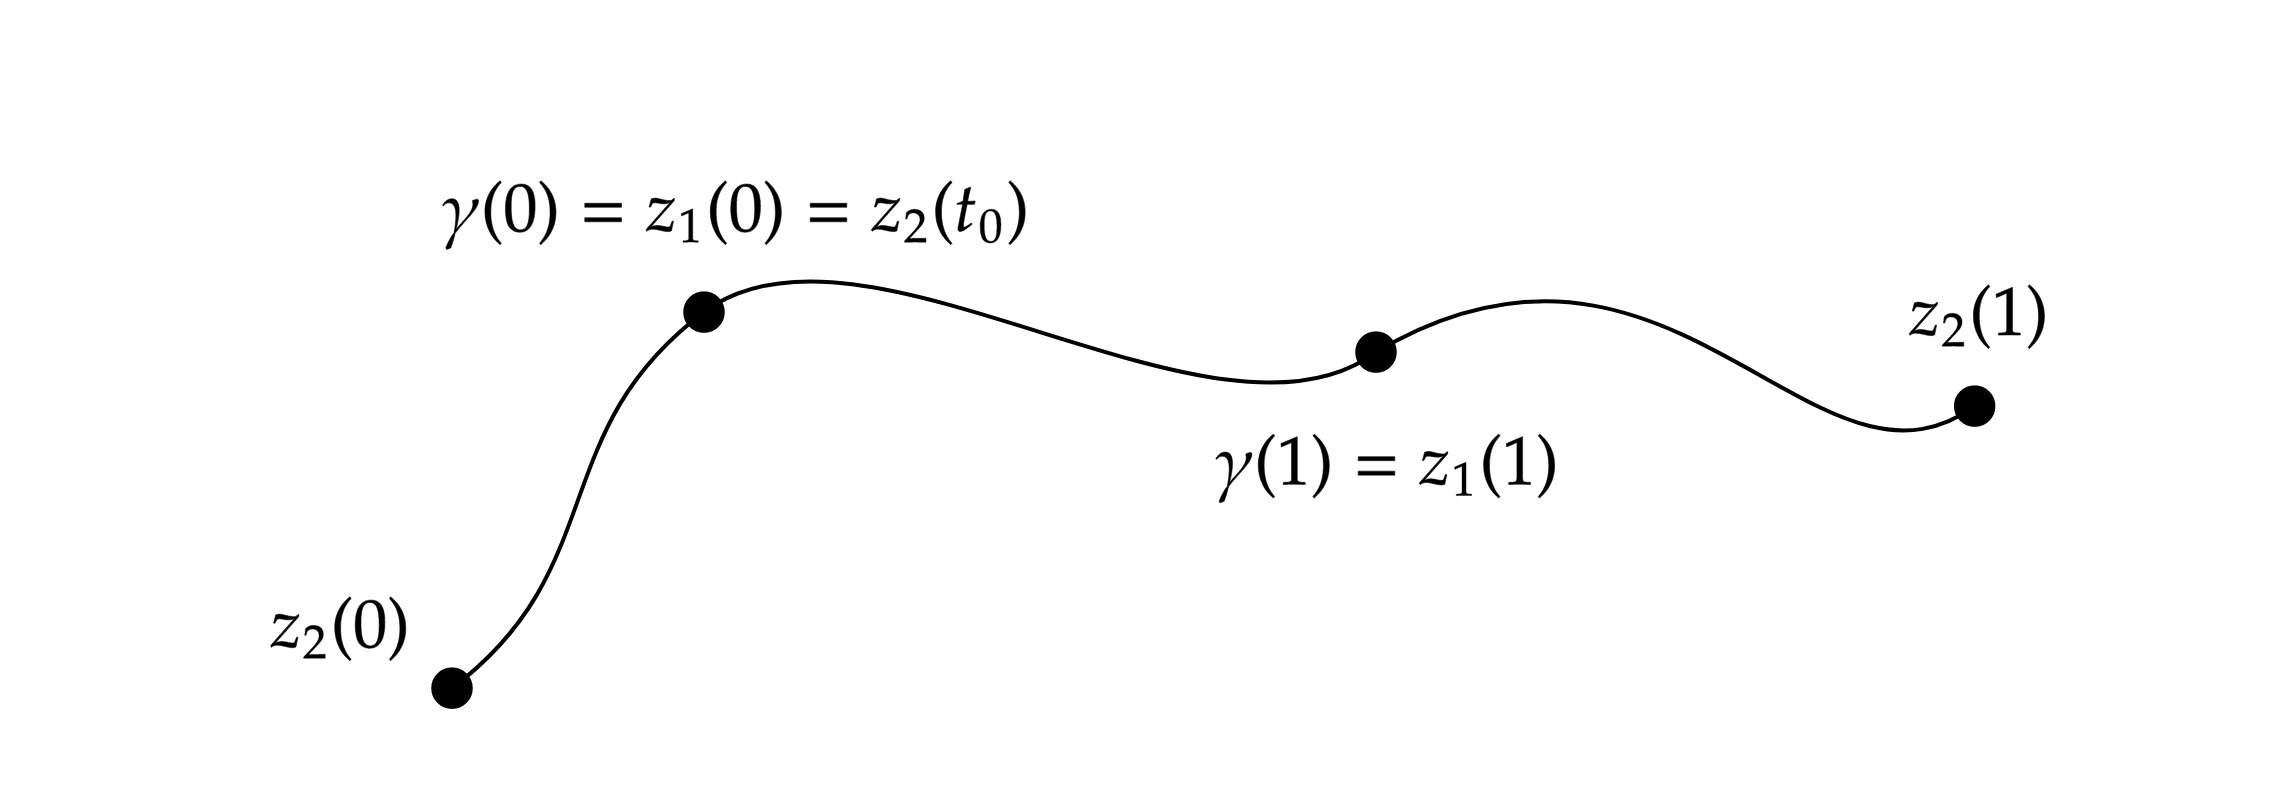
\includegraphics[width = .8\textwidth]{curv02} 
\caption{Case $z_1(1)=\gamma(1)\neq z_2(1)$.}
\label{fig:subim1}
\end{subfigure}
\begin{subfigure}[h]{1\textwidth}
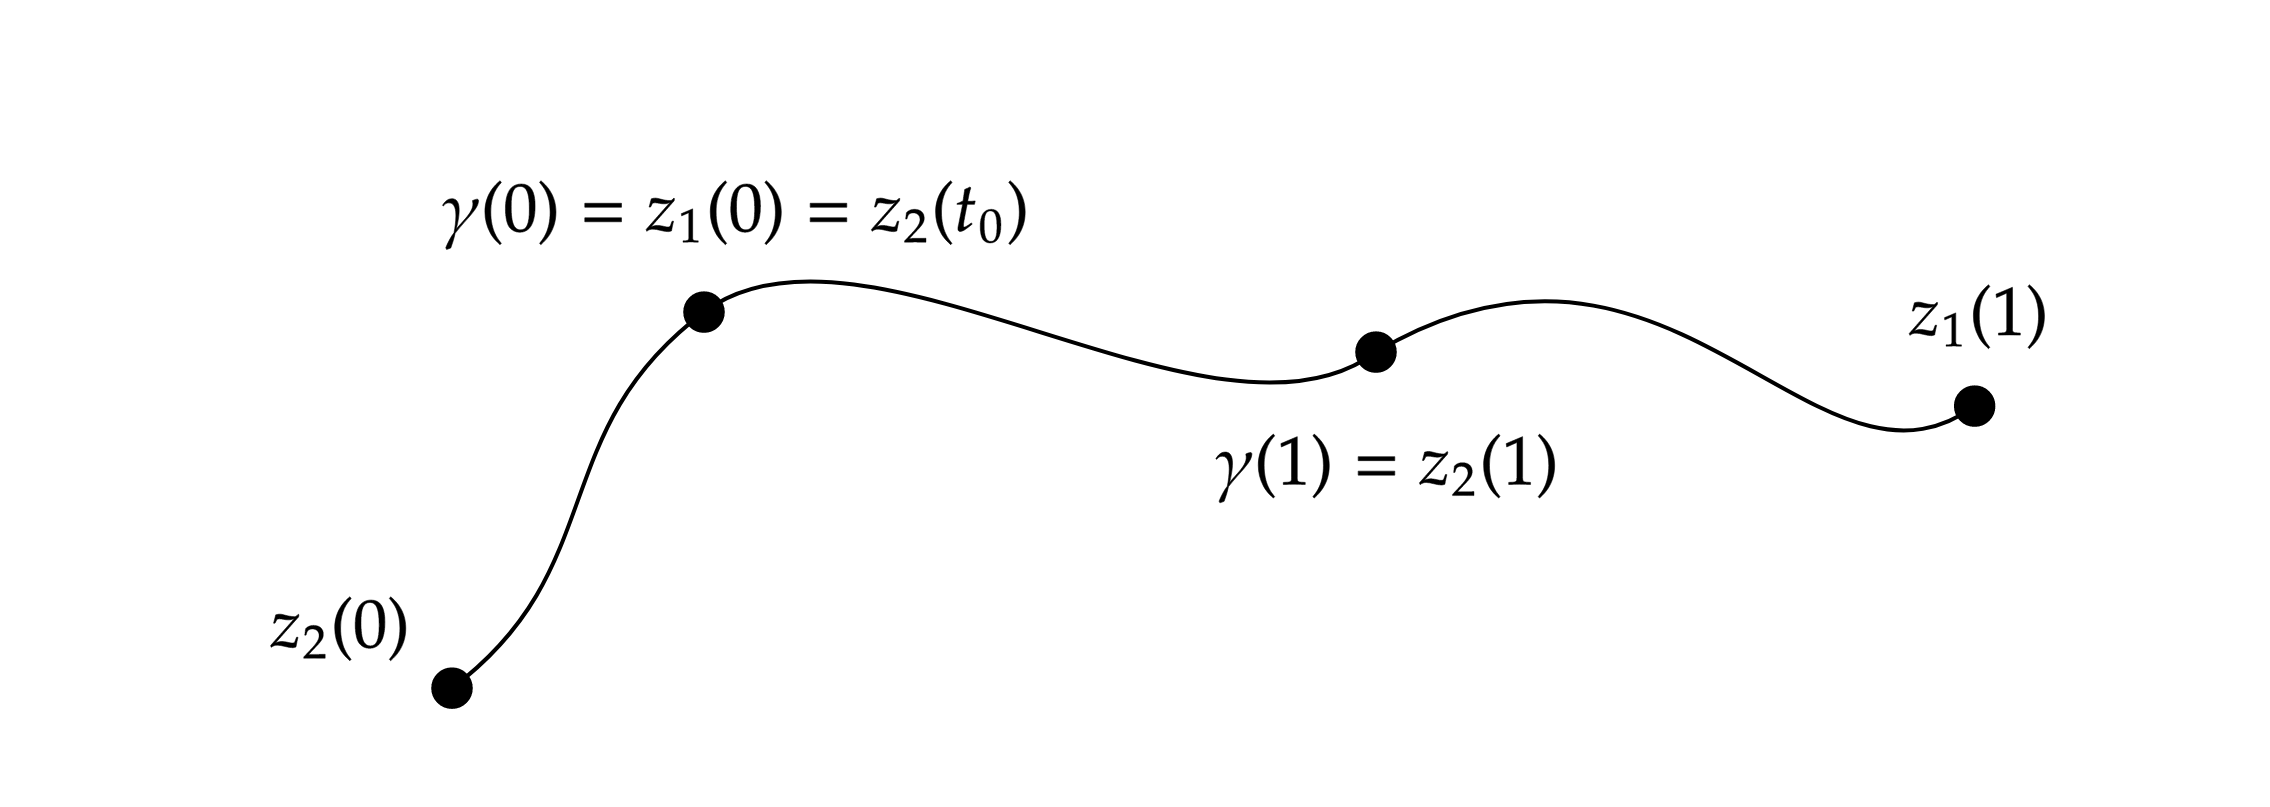
\includegraphics[width =.8 \textwidth]{curv01}
\caption{Case $z_1(1)\neq \gamma(1)=z_2(1)$.}
\label{fig:subim2}
\end{subfigure}

\begin{subfigure}[h]{1\textwidth}
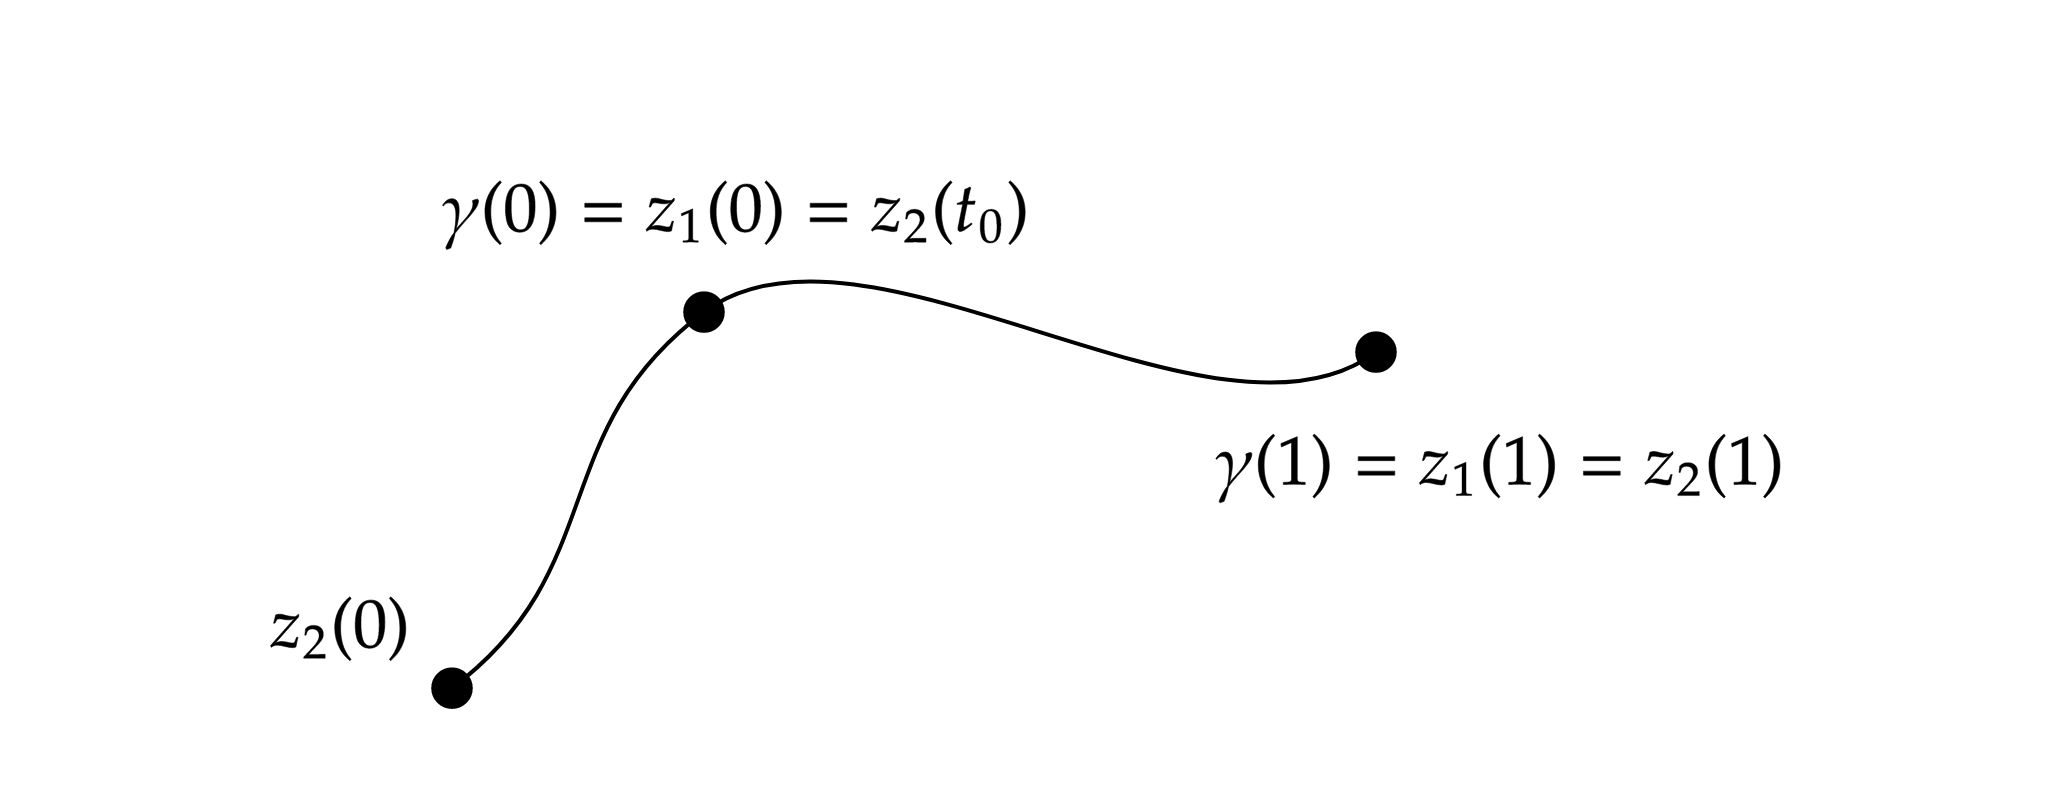
\includegraphics[width = .8\textwidth]{curve3}
\caption{Case $z_1(2)= \gamma(1)=z_2(1)$.}
\label{fig:subim3}
\end{subfigure}
\caption{Finding and analytical path containing $z_1$ and $z_2$.}
\label{fig:image2}
\end{figure}


 Now, if there are more points at which $z_1$ and $z_2$ intersect than those contained in $\gamma$, we find another subpath $\gamma_2$ contained in both $z_1$ and $z_2$. In this case, since $\gamma$ and $\gamma_2$ have the same endpoints as those of $z_1$ and $z_2$, there cannot be more intersections of $z_1$ and $z_2$ than those at the points of $\gamma$ and $\gamma_2$. Similarly as in the previous case, parametrizing consecutively, and in an adequate order, $\gamma,\gamma_2$ and subpaths of $z_1$ or $z_2$ we may construct a path containing $z_1$ and $z_2$. Up to a change of orientation, in this case the setting of the curves will look like in Figure \ref{fig:finalpaths}. As can be seen, in this case the path containing both $z_1$ and $z_2$ will be an analytical closed curve.
 
 \begin{figure}[h!]
	\centering  
  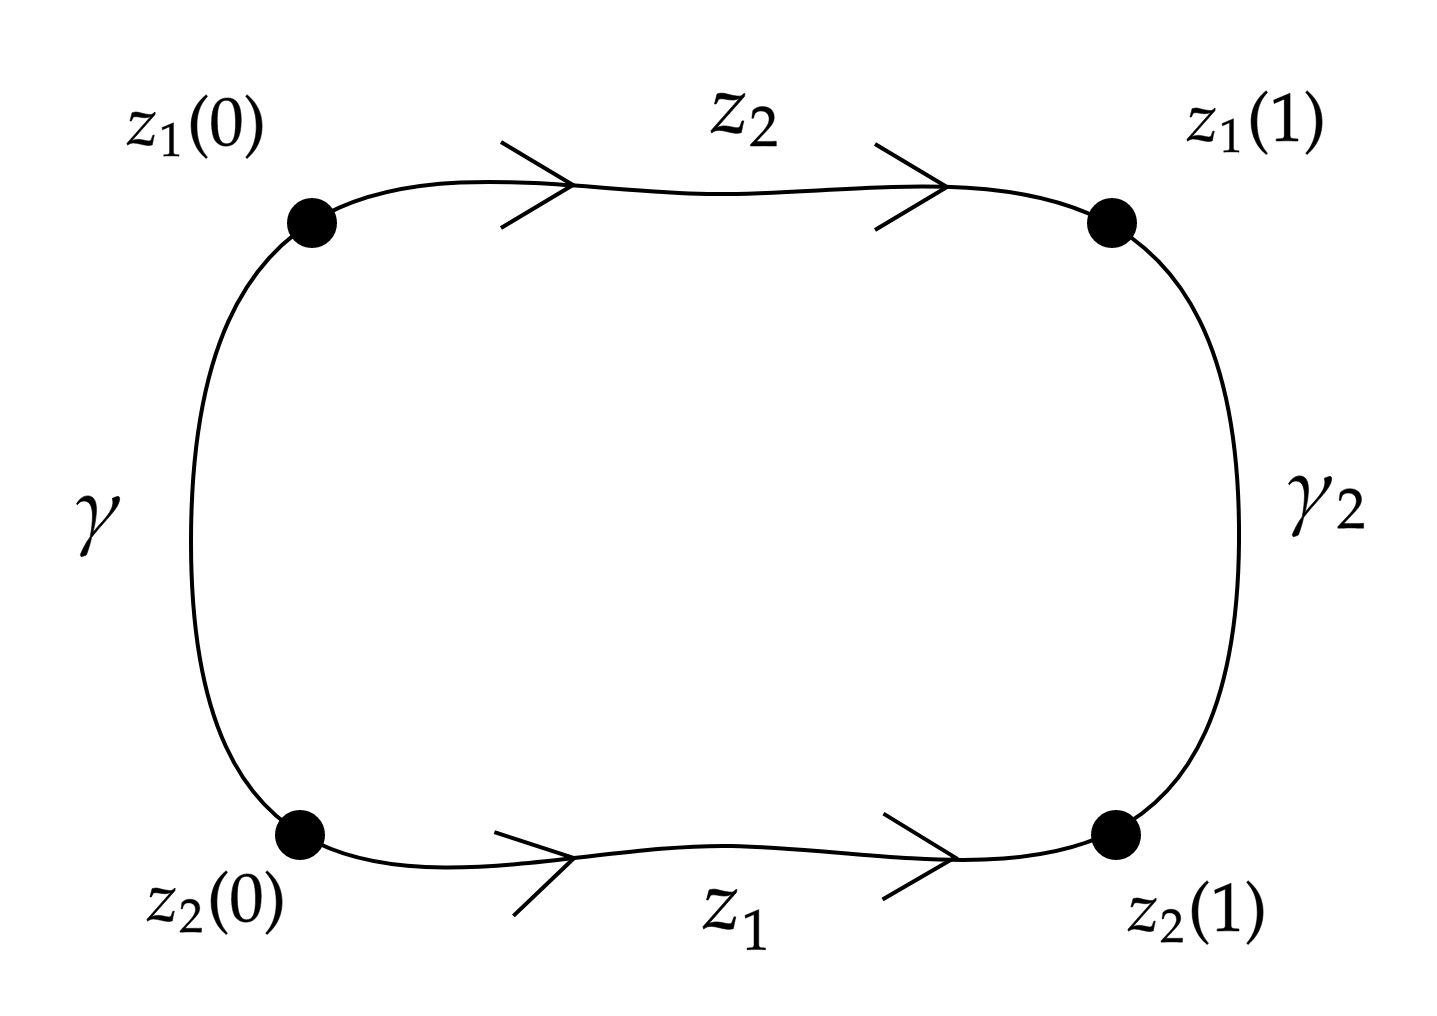
\includegraphics[scale=.18]{finalpaths}
  \caption{}
  \label{fig:finalpaths}
\end{figure}
\end{proof}

\section{The theory of currents}\label{corrientes}

\subsection{Basic definitions}

General references for notions on differential forms and integration over manifolds are \cite{spivak} and \cite{bredon}, in the case of the theory of currents we follow \cite{fornaes} and \cite{demailly}.\\

\subsubsection{The case of real manifolds}
Consider an oriented differentiable manifold $M$ of dimension $n$ and denote by $\mathcal{E}^p(M)$ the space of $p$-forms on $M$ of class $C^\infty$. Then, given local coordinates $(x_1,x_2,\dots,x_n)$ near a point $a\in M$, an element $\omega\in\mathcal{E}^p(M)$ can be written as
$$\omega(x) = \sum_{|I|=p} u_I(x)\,dx_I,$$
where $I=(i_1,\dots,i_p)$ varies over all integer coordinates satisfying $1\leq i_1 < i_2 < \cdots < i_p \leq n$, $I$ is a multi-index and $|I|$ equals the number of components of $I$. Also, $dx_I \coloneqq dx_{i_1} \wedge \cdots \wedge dx_{i_p}$ and the functions $u_I$ are required to be infinitely differentiable. The space $\mathcal{E}^p(M)$ is equipped with the topology generated by the family of seminorms
\begin{equation}\label{seminorms}
p_{L,s}(\omega) = \sup_{x\in L} \max_{|I|=p,|\alpha| \leq s} |D^\alpha u_I(x)|,
\end{equation}
where $L\subset M$ is compact, $s\geq 0$, $\alpha = (\alpha_1,\dots,\alpha_n)$ runs over $(\mathbb{Z}^+)^n$, $|\alpha|=\alpha_1+\cdots +\alpha_n$ and $D^{\alpha} = \partial^{|\alpha|}/\partial x_1^{\alpha_1}\dots \partial x_n^{\alpha_n}$ is a derivation of order $|\alpha|$. The reader must notice that the previous topology is similar as the one given to the space of test functions in distribution theory. Denote by $\mathcal{D}^p(M) \subset \mathcal{E}^p(M)$ the subspace of $p$-differential forms with compact support in $M$, equipped with the induced topology.

\begin{mydef}{}{}
The {\bf space of $p$-currents} $\mathcal{D}_p(M)$ is defined as the dual of $\mathcal{D}^{n-p}(M)$.
\end{mydef} 
\nomenclature[53]{$\mathcal{D}_p(M)$}{The space of $p$-currents on $M$}
If $T$ is a $p$-current and $\omega$ is an $(n-p)$-form in its domain, then $T(\omega)$ is conviniently written as $\langle T, \omega\rangle$. The {\bf support} of a current $T\in \mathcal{D}_p(M)$, denoted as $\supp\,T$, is defined as the smallest closed set $K\subset M$ such that the restriction of $T$ to $\mathcal{D}^{n-p}(M\setminus K)$ is identically zero.\\

Any $p$-form $\eta \in \mathcal{E}^p(M)$ can be identified with a unique $p$-current defined by 

$$\langle T_\eta , \omega \rangle = \int_M \eta \wedge \omega, \quad \omega \in \mathcal{D}^{n-p}(M).$$

Notice that $\eta \wedge \omega$ has compact support so the previous definition makes sense.\\

%We need to stress that any real valued continuous function with compact support contained in a domain $D \subset \mathbb{C}$, and more specifically in a relatively compact set $K\subset D$, is a point of accumulation of $\mathcal{E}^0(K)$ with the $\sup$ norm $\|\cdot\|_\infty$, see for example \cite[Lemma 3.7.3]{ransford}. Hence, any element in the dual of $\mathcal{E}^0(K)$ can be extended to the set of continuous funtions on $K$, using the $\sup$ norm. 
Any continuous linear functional on the set of continuous functions with compact support in a relatively compact set $K\subset D$, equipped with the $\sup$ norm $\|\cdot\|_\infty$, is defined on $\mathcal{E}^0(K)$. By the Riesz Representation Theorem, $\mathcal{D}_n(M)$ contains the set of Radon measures on $M$.\\

Some operations on differential forms can be defined analogously on currents. Let us begin, for example, with the {\bf exterior derivative}. Let $T\in \mathcal{D}_p(M)$, and define $dT\in \mathcal{D}_{p+1}(M)$ pointwisely by
$$\langle dT,\omega\rangle = (-1)^{p+1}\langle T , d\omega \rangle \quad \forall\, \omega \in \mathcal{D}^{n-p-1}(M).$$

Although we do not want to discuss further details, it is of course necessary to show that $dT$ is continuous to ensure that it is a current, however this follows from the fact that $T$ is a current and that $d:\mathcal{D}^p(M)\rightarrow \mathcal{D}^{p+1}(M)$ is continuous with the topology we defined at the beginning, that is, the topology generated by the family of seminorms defined in \ref{seminorms}.\\

Now, let $f:M_1\rightarrow M_2$ be a $C^\infty$ map between manifolds $M_1,M_2$ of respective dimensions $m_1,m_2$. Suppose that $f^*\omega\in \mathcal{D}^p(M_1)$ for every $\omega\in \mathcal{D}^p(M_2)$, then if $T\in \mathcal{D}_{n-p}(M_1)$ we may define a current $f_*T\in \mathcal{D}_{n-p}(M_2)$ pointwisely as
$$\langle f_*T,\omega\rangle = \langle T,f^*\omega\rangle \quad \forall \,\omega \in \mathcal{D}^p(M_2),$$
this current is called the {\bf direct image} of $T$ by $f$.\nomenclature[54]{$f_*$}{The direct image morphism induced by $f$} Notice that if $f$ is a proper map then $f^*\omega\in \mathcal{D}^p(M_1)$ whenever $\omega\in \mathcal{D}^p(M_2)$. However, we can work with a weaker condition, given a current $T$, by simply asking the restriction of $f$ to $\supp \,T$ to be proper, which means that $\supp\, T \cap f^{-1}(K)$ is compact for every compact subset $K\subset M_2$. In this case the pairing $\langle T, f^{*}\omega\rangle$ makes sense and the current $f_*T$ may be defined as before. Notice that in this way only $f_*T$ can be guaranteed to exists, that is, if $S$ is another current, $f_*S$ might not be defined.\\

It is easy to see that the $d$ operator commutes with $f_*$ since for $\omega \in \mathcal{D}^{p-1}(M)$
$$\langle d \, f_*T ,\omega \rangle =(-1)^{p+1} \langle f_*T,d\omega \rangle = (-1)^{p+1} \langle T,d(f^*\omega) \rangle = \langle dT,f^*(\omega) \rangle = \langle f_*dT,\omega \rangle.$$

To end this section, suppose that $f:M_1 \rightarrow M_2$ is a submersion, that is, a surjective map such that for every $x\in M_1$ the differential map $d f : T_{M_1,x} \rightarrow T_{M_2,f(x)}$ is surjective, where $T_{M_1,x},T_{M_2,f(x)}$ are the tangent spaces at $x$ and $f(x)$, respectively (see \cite{epstein} for standard background in differential geometry). Then it is possible to define a \emph{push-forward} $f_*$ of differential forms, this operation is called {\bf integration along/over the fibers} of $f$.\\

We describe, based on $\cite{sternin}$, the construction of this morphism in the next simplest case. Suppose $\pi:E \rightarrow M$ is a fiber bundle with fiber $F$ (see \cite{bott}). Suppose $E$ has real dimension $n$ and that $F$ has real dimension $k$. Denote by $d\pi$ the differential of $\pi$. A vector $v\in T_{E,p}$ is said to be {\bf vertical} if $d\pi(v)=0\in T_{M,\pi(p)}$. Let $n\geq p \geq k$ and $\omega\in \mathcal{D}^p(E)$, also take $Y=(y_1,\dots,y_{p-k})\in T_{M,x}^{p-k}$, then define a $k$-form $\varphi_Y(\omega)$ on $\pi^{-1}(x)$ for $x\in M$ as follows
$$\varphi_Y(\omega)(v_1,v_2,\dots,v_k) = \omega(y_1^*,y_2^*,\dots,y_{p-k}^*,v_1,\dots,v_k),$$
where $y_j^*$ satisfies $d\pi(y_j^*)=y_j$ for each $j$ and $\{v_1,\dots,v_k\}$ are tangent vectors in $T_{E,e}$ for some $e\in \pi^{-1}(x)$. Finally, the {\bf integral of $\omega$ along the fibers} of $\pi$, denoted $\pi_*\omega$, is defined as
\begin{equation}\label{integral_along}
\pi_*\omega(y_1,\dots,y_{p-k}) = \int_{\pi^{-1}(x)} \varphi_Y(\omega).
\end{equation}

Notice that, since $\omega$ has compact support, we do not need $F$ to be a compact manifold. In general, $f_*\omega$ is defined similarly, however for our purposes we actually only need the case $\pi:\mathbb{C}^2\rightarrow \mathbb{P}^1$ which is a complex vector bundle, see the next subsection. We remark that if $r=m_1-m_2\geq 0$ and $\omega \in \mathcal{D}^{p}(M_1)$ then $f_*\omega\in \mathcal{D}^{p-r}(M_2)$, where of course $p\geq r$. 

\begin{myrmk}{}{nh} 
If $f:M_1\rightarrow M_2$ is a submersion, it can be checked that $T_{f_*\omega} = f_*(T_{\omega})$, where $T_{f_*\omega}$ is the current induced by $f_*\omega$ and $f_*(T_{\omega})$ is the direct image of $T_{\omega}$ by $f$, see \cite[(2.15) Special case]{demailly}. It is usual de identify differential forms with their induced currents, hence one may simply write $\omega$ instead of $T_\omega$, and so $f_*\omega$ may denote the integral of $\omega$ along the fibers of $f$ or the direct image of $T_\omega$, depending on the context.
\end{myrmk}

Finally, integration along the fibers also can be used to define the so called {\bf inverse image} $f^*T\in \mathcal{D}_p(M_1)$ of a current $T\in \mathcal{D}_p(M_2)$, which is defined by
$$\langle f^*T,\omega \rangle = \langle T,f_*\omega \rangle, \qquad \forall \, \omega \in D^{m_1-p}(M_1)=D^{m_2-p+r}(M_1).$$
\nomenclature[55]{$f^*$}{The inverse image morphism induce by $f$}
It can be checked that $d$ commutes with integration along the fiber \cite[Theorem 6.14.1]{bott}, hence we have
$$\langle d(f^*T),\omega\rangle = (-1)^q \langle f^*T,d\omega\rangle = (-1)^q \langle T,f_* d\omega\rangle = (-1)^q \langle T, df_*\omega \rangle = \langle f^*(dT),\omega \rangle,$$
which means that exterior derivative commutes with the inverse image. Another important property of the inverse image $f^*$ is that {\it it is an isomorphism onto its image}, see \cite[Proposition 3.2]{fornaes}.\\

As a last property, let $\omega$ be a $p$-form on $M_1$ and $\eta$ be a $n-p$-form on $M_2$, then
\begin{align*}
\langle f^* T_{\eta}, \omega \rangle &= \langle T_\eta , f_*\omega\rangle\\
&= \langle T_{f_*\omega},\eta \rangle \\
&= \langle f_*T_\omega,\eta \rangle \quad \text{by Remark \ref{rm:nh}}\\
&= \langle T_\omega,f^*\eta\\
&= \langle T_{f^{*}\eta},\omega \rangle.\\
\end{align*}
In short,
\begin{equation}\label{laecu}
f^*T_\eta = T_{f^*\eta}.
\end{equation}

\subsubsection{The case of complex manifolds}
Suppose that $M$ is a {\emph complex manifold} of dimension $n$ and that $z=(z_1,z_2,\dots,z_n)$ are local holomorphic coordinates. Then any {\bf $r$-form} $\omega$ can be written locally as 
$$\omega(z) = \sum_{|I|+|J|=r} u_{I,J}(z)\, dz_I\wedge \overline{z}_J,$$
where $u_{I,J}$ are infinitely differentiable functions with complex values and $I,J$ are multi-indices. We say that a $r$-form is of {\bf bidegree} $(p,q)$ if $u_{I,J}=0$ whenever $|I|\neq p$ or $|J| \neq q$, the set of all $(p,q)$-forms is denoted as $\mathcal{E}^{p,q}(M)$. The space $\mathcal{E}^r(M,\mathbb{C})$ of $r$-forms can be decomposed as
$$\mathcal{E}^r(M,\mathbb{C}) = \bigoplus_{p+q=r} \mathcal{E}^{p,q}(M),$$
where of course $r,p,q\geq 0$.\\

We can give a topology to $\mathcal{E}^r(M,\mathbb{C})$ and $\mathcal{E}^{p,q}(M)$ exactly in the same way as in the real case. We define the subspaces $\mathcal{D}^r(M,\mathbb{C})\subset \mathcal{E}^r(M,\mathbb{C})$ and $\mathcal{D}^{p,q}(M) \subset \mathcal{E}^{p,q}(M)$ of currents with compact support, equipped with the induced topology.\\

\begin{mydef}{}{}
The space of currents $\mathcal{D}_{p,q}(M)$ of bidegree $(p,q)$ and of bidimension $(n-p,n-q)$ is defined as the dual space of $\mathcal{D}^{n-p,n-q}(M)$.
\end{mydef}
\nomenclature[59]{$\mathcal{D}_{p,q}(M)$}{The space of $(p,q)$ currents on a complex manifold $M$}
We will use the generalized Laplacian in the next subsection. In  local coordinates, if $\omega = \sum_{I,J} u_{I,J} dz_{I}\wedge d\bar z_{J}$ then the differential operators $\partial,\bar{\partial}$ are defined as
$$\partial\,\omega = \sum_{I,J}\sum_{1\leq k \leq n} \frac{\partial u_{I,J}}{\partial z_k} \,dz_k\wedge dz_{I}\wedge d\bar z_{J},$$
\nomenclature[60]{$\partial,\bar \partial$}{Differential operators on complex forms}
$$\bar \partial\,\omega = \sum_{I,J}\sum_{1\leq k \leq n} \frac{\partial u_{I,J}}{\partial \bar{z}_k} \,d\bar{z}_k\wedge dz_{I}\wedge d\bar z_{J}.$$

Next, define $d = \partial + \bar \partial$ and $d^c = i(\bar \partial - \partial)/(2\pi)$. The operator $dd^c = \frac{i}{\pi}\partial \bar \partial$ is a normalized generalization of the Laplacian $\Delta$. These operators can be extended to currents as follows: if $T$ is a $(p,q)$-current and $\omega$ is a $(p,q)$-form, then the currents $\partial T$ and $\bar \partial T$ are defined pointwisely as
$$ \langle \partial T, \omega\rangle = (-1)^{p+q+1}\langle T,\partial \omega \rangle,$$
and 
$$ \langle \bar\partial T, \omega\rangle = (-1)^{p+q+1}\langle T,\bar \partial \omega \rangle.$$
Then, $dd^c T$ is defined by
$$ \langle dd^c T , \omega \rangle = \frac{i}{\pi} \langle T , \partial \bar \partial \omega \rangle.$$
\nomenclature[61]{$dd^c$}{A generalization of the Laplacian operator}
As in the real case, if $f:M_1\rightarrow M_2$ is a holomorphic map between complex manifolds of respective dimensions $m_1,m_2$, we can define the direct image $f_*T$ of a $(p,q)$-current $T$ in $M_1$, whenever $f$ restricted to $\supp\, T$ is proper. This current acts pointwisely as
$$\langle f_*T,\omega\rangle = \langle T , f^*\omega\rangle \quad \forall \,\omega \in D^{m_1-p,m_2-p}(M_1).$$

We will be interested specially in the projective map $\pi: \mathbb{C}^2\setminus\{(0,0)\} \rightarrow \mathbb{P}^1$ given by $\pi(z,w)=[w/z]$ if $z\neq 0$ and $\pi(z,w) = [\infty]$ otherwise. Notice that each fiber $\pi^{-1}([w/z])$ is linearly isomorphic to $\mathbb{C}^2$. Actually, $\pi$ is a complex vector bundle. As before, we can define the morphism of integration along the fiber $\pi_*: \mathcal{D}^{2,2}(\mathbb{C}^2) \rightarrow \mathcal{D}^{1,1}(\mathbb{P}^1)$ and the {\it pull-back} morphism $\pi^*: \mathcal{D}_{0,0}(\mathbb{P}^1) \rightarrow \mathcal{D}_{0,0}(\mathbb{C}^2)$ is defined as its transpose.
%
%To define $\pi_*$ consider a trivial complex bundle $E= U\times \mathbb{C}^1$ where $U\subset \mathbb{P}^1$ is a proper open set. Any form in $\mathcal{D}^{2,2}(E)$ is a linear combination of forms which contain a factor $dz\wedge d\bar{z}$. Hence, it is sufficient to define $\pi_*$ on the forms which can be written as $(\pi^* \varphi)\wedge f(p,z,\bar{z}) dz\wedge d\bar{z}$, where $\varphi$ is a $(1,1)$-form on $\mathbb{P}^1$ and $\pi^*\varphi$ denotes the standard pull-back. These forms are mapped under $\pi_*$ as follows

%of the following two types of forms: the type (I) forms are those which do not contain a factor $dz\wedge d\bar{z}$ and type (II) forms are those which do. A type I form can be written as $(\pi^* \phi)\wedge f(p,w)dw$ where $w$ stands either for $z$ or $\bar{z}$, $\phi$ is a form on $M\ni p$ and $f$ has compact support. Also, $(\pi^* \phi)$ denotes the standard pull-back of forms. So first, $\pi_*$ is defined as $0$ on type I forms. Similarly, type II forms can be written as $(\pi^* \phi)\wedge f(p,z,\bar{z}) dz\wedge d\bar{z}$, and thess forms are mapped under $\pi_*$ as follows
%$$(\pi^* \phi)\wedge f(p,z,\bar{z}) dz\wedge d\bar{z} \mapsto \phi \int_{\mathbb{C}}f(p,z,\bar{z}) dz\wedge d\bar{z}.$$
%
%It can be checked that if $\omega\in \mathcal{D}^{2,2}(E)$ and $\pi_*\omega$ is identified with the current it induces, this current coincides with the direct image of $\omega$ (as a current) by $\pi$ as defined in the previous section.\\
%
%Finally, $\pi_*$ is defined on $\mathcal{D}^{2,2}(\mathbb{C}^2)$ by using partitions of unity to write any form as sum of forms with support contained in a coordinate neighbourhood.

\subsection{Application to complex dynamics}\label{sect3}

This subsection is mainly based on \cite{demarco}, \cite{hubbard}, \cite{bott} and \cite{berteloot}.\\

Let $\pi:\mathbb{C}^2\setminus\{(0,0)\} \rightarrow \mathbb{P}^1$ be the canonical projection.
\begin{mydef}{}{}
Let $U\subset \mathbb{P}^1$ be a proper open set. A {\bf holomorphic section} of $\pi$ defined on $U$ is a holomorphic function $\sigma:U \rightarrow \mathbb{C}^2\setminus\{(0,0)\}$ such that $\pi \circ \sigma$ is the identity function on $U$.
\end{mydef}

It is sufficient to think that $U$ in the previous definition is either $\mathbb{P}^1\setminus \{\infty\}$ or $\mathbb{P}^1\setminus\{0\}$. Moreover, as a consequence of the Maximum Modulus Principle there cannot be holomorphic sections defined over all $\mathbb{P}^1$. Nontheless, we will treat with non-holomorphic sections, that is, functions $\widehat{\sigma}$ such that $(\pi \circ \widehat{\sigma})(z)=z$ for every $z\in \mathbb{P}^1$.\\

Now define $V(Z,W) \coloneqq  \log \frac{|Z\wedge W|}{\|W\|}$ for $Z,W \in \mathbb{C}^2\setminus\{0\}$. It is easily shown that $V(Z,aW) = V(Z,W)$ for any $a\in \mathbb{C}^*$.\\

\begin{myprop}{}{propo_potenshial}
Let $\mu$ be a positive measure on $\mathbb{P}^1$. Define the potential function $U_\mu:\mathbb{C}^2\rightarrow \mathbb{R}\cup\{-\infty\}$ by
$$U_\mu(Z) = \int_{\mathbb{P}^1} V(Z,\widehat{\sigma}(w)) \, d\mu(w),$$
for $Z\in \mathbb{C}^2$ and where $\widehat{\sigma}$ is a non-holomorphic section of $\pi$ defined over all $\mathbb{P}^1$.
Then if $\sigma$ is a holomorphic section of $\pi$ defined on $U\subset \mathbb{P}^1$, we have 
$$dd^c (U_\mu\circ \sigma) = \mu,$$
where the equality must be interpreted in the sense of currents.
\end{myprop}

A proof of Proposition \ref{pr:propo_potenshial} can be found in \cite[Theorem VII.9]{berteloot}. See also \cite[Theorem 3.7.4]{ransford}.\\

\begin{mytheo}{}{teohubbard}
Let $f:\mathbb{P}^1 \rightarrow \mathbb{P}^1$ be a rational function and $F:\mathbb{C}^2 \rightarrow \mathbb{C}^2$ a lift of $f$. Let $G^F$ the Green function associated to $F$ and $\mu_f$ be the measure of maximal entropy for $f$, then
$$dd^c G^F = \pi^*(\mu_f).$$
\end{mytheo}

Notice that in Theorem \ref{th:teohubbard} $dd^c$ is the operator defined for functions on $\mathbb{C}^2$. A proof of Theorem \ref{th:teohubbard} can be found in \cite[Theorem 4.1]{hubbard}.\\

\begin{proof}[Proof of Proposition \ref{pr:generallaplacian}]
For convenience let us recall that the $F$-potential for $\mu$ is
$$U_{F,\mu} (z) = \int_{\mathbb{P}^1} \Phi_F(z,w)\,d\mu(w),$$

where $\Phi_F(z,w)$ is given by

$$\Phi_F(z,w) = \log |Z\wedge W| -G^F(Z)-G^F(W), \qquad Z\in \pi^{-1}(z),\,W\in \pi^{-1}(w).$$
In Section \ref{seccionweighted} was shown that the previous formula of $\Phi_F$ is independent of the points $Z\in \pi^{-1}(z)$ and $W\in \pi^{-1}(w)$.\\

Let $U_1=\mathbb{P}^1 \setminus \{\infty\}\cong \mathbb{C}$ and $U_2 = \mathbb{P}^1\setminus\{0\}$. Since each $U_i\subset \mathbb{P}^1$ is a coordinate open set we know that $dd^c$ has an explicit expression on each one. Moreover, using partitions of unity we can decompose any differential form $\omega$ defined on $\mathbb{P}^1$ as $\omega = \varphi_1+\varphi_2$, where $\supp\, \varphi_i$ is a compact subset of $U_i$ for $i=1,2$. Because $dd^c\omega = dd^c\varphi_1+dd^c\varphi_2$, it suffices to show that the result is true on $U_1$ and $U_2$ separately. It is also sufficient to treat the case of $U_1$ only.\\

Let $\sigma:U_1\subset \mathbb{P}^1 \rightarrow \mathbb{C}^2$ be the holomorphic section of $\pi$ given by $\sigma([z/1])=(1,z)$, and let $\widehat{\sigma}:\mathbb{P}^1 \rightarrow \mathbb{C}^2$ be a non-holomorphic section of $\pi$. From the identity

$$\log |Z\wedge W| -G^F(Z)-G^F(W) = \log \frac{|Z\wedge W|}{\|W\|}-G^F(Z)-(G^F(W)-\log\|W\|),$$
 
we can rewrite the potential $U_{F,\mu}$ as
\begin{align*}
U_{F,\mu}(z) &= \int_{\mathbb{P}^1}V(\sigma(z),\widehat{\sigma}(w)) \,d\mu(w) -G^F(\sigma(z))\mu(\mathbb{P}^1)-\int_{\mathbb{P}^1}G^F(\widehat{\sigma}(w))-\log\|\widehat{\sigma}(w)\| \,d\mu(w)\\
&= U_{\mu}(\sigma (z))-G^F(\sigma(z))\mu(\mathbb{P}^1)-\int_{\mathbb{P}^1}G^F(\widehat{\sigma}(w))-\log\|\widehat{\sigma}(w)\| \,d\mu(w),
\end{align*}
for $z\in U_1\subset \mathbb{P}^1$.\\

From Proposition \ref{pr:propo_potenshial} we know that
$$dd^c U_{\mu}(\sigma (z)) = \mu.$$

In order to obtain $dd^c U_{F,\mu}$, it only remains to calculate $dd^c G^F(\sigma(z))$. Let $\pi^*$ denote the standard pull-back by $\pi$. Then, due to the fact that $\pi$ is holomorphic, it commutes with $dd^c$, so
$$\pi^* dd^c_{\mathbb{P}^1} G^F(\sigma(z)) = dd^c_{\mathbb{C}^2\setminus\{0\}} \pi^*G^F\circ \sigma,$$
where we used subscripts to emphasize that the operators $dd^c$ on each side of the equation are defined on different manifolds. Notice that $(\pi^* G^F\circ \sigma)(Z) = G^F((\sigma\circ \pi)(Z)) = G^F(\lambda(Z)\cdot Z)$, where $\lambda:\mathbb{C}^2\setminus\{(0,w)\,:\,w\in \mathbb{C}\} \rightarrow \mathbb{C}$ is given by $\lambda(z,w)=1/z$.

If we use the property in \eqref{equgreen01} we further obtain
\begin{equation}\label{lachida}
\pi^* dd^c_{\mathbb{C}^2\setminus\{0\}} G^F(\sigma(z)) = dd^c_{\mathbb{C}^2\setminus\{0\}} G^F(Z) + dd^c_{\mathbb{C}^2\setminus\{0\}} \log|\lambda(Z)|.
\end{equation}
Also, let $\Delta = \frac{\partial^2}{\partial x^2}+\frac{\partial^2}{\partial y^2}$, then
\begin{align*}
dd^c_{\mathbb{C}^2\setminus\{0\}}\log \lambda(Z) &= \frac{i}{\pi} \frac{\partial^2}{\partial z\partial \bar z} \log(1/|z|) dz\wedge d\bar z\\
&= \frac{i}{4\pi}\Delta(-\log\sqrt{x^2+y^2})(-2i\,dx\wedge dy)\\
&= -\Delta \frac{\log\sqrt{x^2+y^2}}{2\pi}\, dx\wedge dy = -\delta_0\, dx\wedge dy,
\end{align*}
where the last equality is explained in \cite[Section 3.D.]{demailly}. This implies that if $\varphi$ is a $(1,1)$-form with compact support in $\mathbb{C}^2\setminus\{(0,0)\}$, then
$$\langle dd^c_{\mathbb{C}^2\setminus\{0\}} \log|\lambda(Z)| , \varphi \rangle = -\int_{0\times \mathbb{C}^*} \varphi.$$
Denote by $[M]$ the current of integration over a manifold $M$, see \cite[Example 2.4]{demailly}. Then $dd^c_{\mathbb{C}^2\setminus\{0\}} \log|\lambda(Z)| = -[0\times \mathbb{C}^*]=-[\pi^{-1}(\infty)]$. Notice that the current of integration over the single point $\{\infty\}$ is $\delta_\infty$. Then, it can be shown that $\pi^*\delta_\infty = [\pi^{-1}(\infty)]$, where this time $\pi^*$ denotes the inverse image of currents, see \cite[Section 2.C.2.]{demailly}. Hence $dd^c_{\mathbb{C}^2\setminus\{0\}} \log|\lambda(Z)| = -\pi^*\delta_\infty$. But we are dealing with differential forms whose support is contained in $U_1=\mathbb{P}^1\setminus\{\infty\}$, so in this case $\delta_\infty= 0$. Recall from Equation \eqref{laecu} that the inverse image of currents is given by the pull-back when it is defined. So, using Theorem \ref{th:teohubbard} and Equation \eqref{lachida}, it is deduced that
$$\pi^* dd^c_{\mathbb{P}^1} G^F(\sigma(z)) = \pi^* (\mu_f-\delta_\infty)=\pi^*\mu_f.$$

Since $\pi^*$ is a monomorphism, we get
$$dd^c_{\mathbb{P}^1} G^F(\sigma(z)) = \mu_f.$$
The previous calculations imply that
$$dd^c_{\mathbb{P}^1} U_{F,\mu} = \mu -\mu(\mathbb{P}^1)\mu_f.$$

\end{proof}

